\newpage
\subsection{2. Kết quả thực nghiệm}
Việc huấn luyện và thực nghiệm mô hình được tiến hành trên nhiều máy chủ khác nhau, với các cấu hình phần cứng như sau:
\begin{itemize}[label={--}, itemsep=1pt]
    \item \textbf{Hệ điều hành:} Debian 11
    \item \textbf{RAM:} từ 192 GiB đến 512 GiB
    \item \textbf{CPU:} Intel Xeon Silver/Gold và AMD EPYC
    \item \textbf{GPU:} Nvidia Quadro RTX 6000 (23 GiB) và Nvidia A40 (45 GiB)
    \item \textbf{Thư viện:} Sử dụng các thư viện phổ biến cho từng tác vụ như:
    \begin{itemize}[label={+}, itemsep=1pt]
        \item Xây dựng các mô hình học sâu: torch (2.9.0), torchvision (0.24.0), torch-geometric (2.7.0), fastkan\footnote{\url{https://github.com/ZiyaoLi/fast-kan}}.
        \item Xử lý ảnh và CNN backbone: torchvision (0.24.0), pillow (12.0.0).
        \item Xử lý văn bản: underthesea (8.3.0) cho tách câu, tokenization và POS tagging; sentence-transformers (5.1.2) cho tạo embedding văn bản.
        \item Xử lý âm thanh: librosa (0.11.0).
        \item Hỗ trợ mô hình máy học truyền thống và các thang đo đánh giá: numpy (2.3.4), pandas (2.3.3), scikit-learn (1.7.2).
    \end{itemize}
\end{itemize}

\subsubsection{2.1. Các thông số cho huấn luyện và kiểm thử}

\paragraph{2.1.1. Tham số mô hình, siêu tham số và kỹ thuật huấn luyện}
\indent\indent Về cấu hình tham số, đề tài áp dụng chiến lược đóng băng toàn bộ kiến trúc CNN backbone trong việc huấn luyện baseline và huấn luyện mô hình MGAT + FastKAN. Ngoài ra, mô hình ngôn ngữ all-MiniLM-L6-v2 cũng được sử dụng ở chế độ đóng băng để trích xuất đặc trưng văn bản. Do đó, tổng số lượng tham số (Total Params) của hệ thống bao gồm cả phần đóng băng và phần có thể huấn luyện (Trainable Params). Chi tiết thống kê tham số cho từng kịch bản cụ thể như sau:

\vspace{0.3cm}
%===================================================================
\textbf{* CNN Baseline:}
\begin{table}[H]
    \centering
    \caption{Thống kê số lượng tham số của các mô hình CNN Baseline}
    \label{tab:CNNBaselineParams}
    \renewcommand{\arraystretch}{1.15}
    \begin{tabular}{lcccc}
        \hline
        \textbf{Mô hình} & \textbf{Trainable Params} & \textbf{Total Params} \\
        \hline
        ResNet18              & 4.1K & 11.2M \\
        RegNetX400MF          & 3.2K & 5.1M \\
        MobileNetV3 Large     & 7.7K & 3.0M \\
        MobileNetV3 Small     & 4.6K & 1.0M \\
        DenseNet121           & 8.2K & 7.0M \\
        ShuffleNetV2 1.0x     & 8.2K & 1.3M \\
        \hline
    \end{tabular}
\end{table}

%===================================================================
\newpage
\textbf{* CNN backbone + MGAT + FastKAN/MLP:}
\begin{table}[H]
    \centering
    \renewcommand{\arraystretch}{1.2}
    \setlength{\tabcolsep}{6pt}
    \caption{\centering Thống kê số lượng tham số của mô hình CNN backbone + MGAT + FastKAN/MLP}
    \begin{tabular}{llcccc}
        \hline
        \textbf{Backbone Model (+ MGAT)} & \textbf{Classifier} & \textbf{Trainable Params} & \textbf{Total Params} \\
        \hline
        % ResNet18
        \multirow{2}{*}{ResNet18} 
        & FastKAN & 4.9M & 38.8M \\
        & MLP & 4.1M & 38.0M \\
        \hline
        % RegNetX400MF
        \multirow{2}{*}{RegNetX400MF} 
        & FastKAN & 4.9M & 32.7M \\
        & MLP & 4.1M & 31.9M \\
        \hline
        % MobileNetV3 Large
        \multirow{2}{*}{MobileNetV3 Large} 
        & FastKAN & 5.1M & 30.8M \\
        & MLP & 4.3M & 30.0M \\
        \hline
        % MobileNetV3 Small
        \multirow{2}{*}{MobileNetV3 Small} 
        & FastKAN & 5.0M & 28.6M \\
        & MLP & 4.2M & 27.8M \\
        \hline
        % DenseNet121
        \multirow{2}{*}{DenseNet121} 
        & FastKAN & 5.2M & 34.8M \\
        & MLP & 4.4M & 34.0M \\
        \hline
        % ShuffleNetV2
        \multirow{2}{*}{ShuffleNetV2 1.0x} 
        & FastKAN & 5.2M & 29.1M \\
        & MLP & 4.4M & 28.3M \\
        \hline
    \end{tabular}
    \label{tab:PipelineFullParams}
\end{table}

%===================================================================
\textbf{* Các siêu tham số và kỹ thuật huấn luyện:}
Quá trình huấn luyện được thực hiện thống nhất với bộ siêu tham số sau:
\begin{itemize}[label={--}, itemsep=1pt]
    \item Epoch: 100.
    \item Batch size: 8.
    \item Accumulation steps: 2 (Kỹ thuật tích lũy gradient này giúp mô phỏng kích thước batch thực tế là 16, cho phép mô hình hội tụ ổn định hơn mà vẫn tiết kiệm bộ nhớ VRAM)
    \item Early Stopping: Cơ chế dừng sớm được kích hoạt với patience = 10. Nếu sau 10 epoch liên tiếp giá trị \textit{validation loss} không cải thiện, quá trình huấn luyện sẽ tự động kết thúc.
    \item Optimizer: \textit{AdamW} với tốc độ học khởi tạo \textit{lr = 1e-4} và trọng số suy giảm \textit{weight\_decay = 1e-5}.
    \item Scheduler: Sử dụng chiến lược \textit{ReduceLROnPlateau} để tự động giảm tốc độ học (factor=0.5) nếu loss không giảm sau 3 epoch (patience=3).
    \item Drop Node (Augmentation): Để tăng khả năng tổng quát hóa của mô hình, tôi áp dụng kỹ thuật loại bỏ ngẫu nhiên các đỉnh ngay trong quá trình huấn luyện. Quy trình bao gồm 2 lượt drop liên tiếp:
    \begin{itemize}[label={+}, itemsep=1pt]
        \item Hình ảnh: Lần 1 (tỷ lệ 0.2), Lần 2 (tỷ lệ 0.3).
        \item Văn bản: Lần 1 (tỷ lệ 0.3), Lần 2 (tỷ lệ 0.4). Đặc biệt, áp dụng ràng buộc min\_not\_drop = 10 để đảm bảo mỗi mẫu luôn giữ lại ít nhất 10 từ khóa quan trọng, tránh làm mất mát hoàn toàn ngữ nghĩa của mô tả.
        \item Âm thanh: Lần 1 (tỷ lệ 0.2), Lần 2 (tỷ lệ 0.3).
    \end{itemize}
    Tỷ lệ drop cao hơn được áp dụng cho văn bản vì số lượng đỉnh của phương thức này chiếm đa số trong đồ thị và có độ biến động cao, trong khi số lượng đỉnh hình ảnh và âm thanh là cố định (lần lượt là 15 hình ảnh và 12 đoạn âm thanh). Thống kê phân bố số lượng từ trong tập huấn luyện được thể hiện tại \textbf{Hình \ref{fig:ThongKeTongSoTu}} và \textbf{Hình \ref{fig:ThongKeTBSoTu}}.
\end{itemize}

\begin{figure}[H]
    \centering
    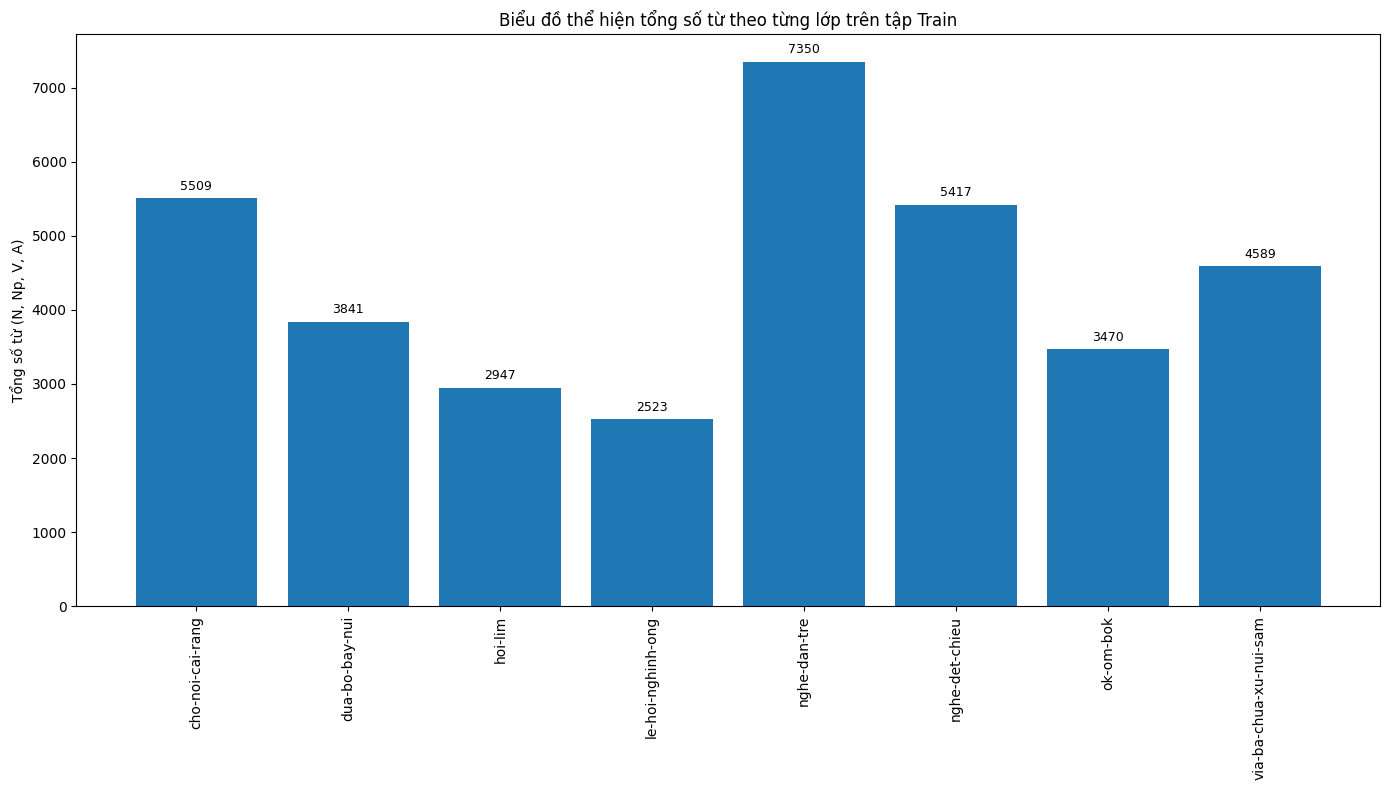
\includegraphics[width=0.9\linewidth]{images/part-02/chap-03/sec-02/ThongKeTongSoTu.png}
    \caption{Biểu đồ thống kê tổng số từ vựng trên tập Train}
    \label{fig:ThongKeTongSoTu}
\end{figure}
\begin{figure}[H]
    \centering
    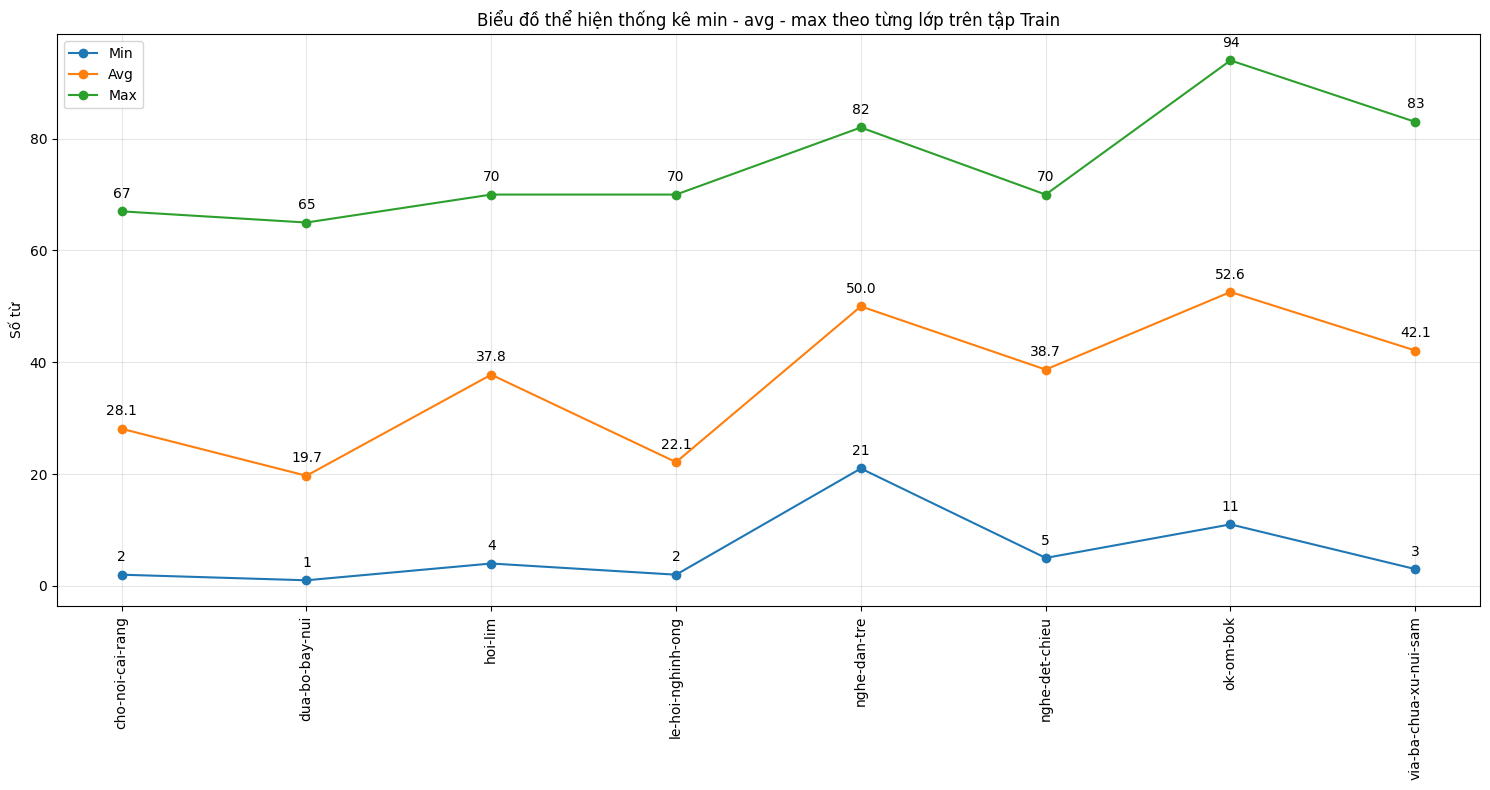
\includegraphics[width=0.9\linewidth]{images/part-02/chap-03/sec-02/ThongKeTBSoTu.png}
    \caption{Biểu đồ thống kê số lượng từ (Min, Avg, Max) trên tập Train}
    \label{fig:ThongKeTBSoTu}
\end{figure}

\paragraph{2.1.2. Chiến lược kiểm thử}
\indent\indent Quy trình kiểm thử tuân thủ nguyên tắc best model checkpoint. Trong quá trình huấn luyện, tại cuối mỗi epoch, nếu giá trị \textit{val\_loss < best\_val\_loss}, trạng thái trọng số của mô hình sẽ được lưu lại. Khi quá trình huấn luyện kết thúc (do hoàn thành 100 epoch hoặc early stopping), hệ thống sẽ tải lại phiên bản trọng số tốt nhất này để thực hiện đánh giá trên tập Test, đảm bảo kết quả phản ánh đúng năng lực của mô hình.\vspace{0.3cm}

Bên cạnh đó, nhằm đảm bảo tính khách quan và độ ổn định của quá trình huấn luyện cũng như các kết quả kiểm thử, đề tài sử dụng ba giá trị \textit{random seed} khác nhau, lần lượt là 1023, 123 và 42 (trong đó seed 42 được sử dụng cho kỹ thuật \textit{drop node}). Kết quả cuối cùng được báo cáo dưới dạng giá trị trung bình của ba lần huấn luyện và kiểm thử độc lập.
\subsubsection{2.2. Kết quả kiểm thử trên các mô hình CNN baseline}
\indent\indent Dưới đây là kết quả kiểm thử chi tiết của sáu mô hình CNN baseline, trong đó các giá trị được lấy từ lần chạy đạt kết quả cao nhất.\vspace{0.3cm}

\textbf{* ResNet18}
\begin{table}[H]
\centering
\renewcommand{\arraystretch}{1.0}
\caption{Classification report của ResNet18 trên CNN baseline}
\label{tab:CRResNet18}
\begin{tabular}{lcccc}
\hline
\textbf{Lớp} & \textbf{Precision} & \textbf{Recall} & \textbf{F1-Score} & \textbf{Support} \\
\hline
cho-noi-cai-rang          & 0.9333 & 0.9333 & 0.9333 & 45 \\
dua-bo-bay-nui             & 0.9574 & 1.0000 & 0.9783 & 45 \\
hoi-lim                    & 0.9333 & 0.9333 & 0.9333 & 45 \\
le-hoi-nghinh-ong          & 0.8108 & 0.6667 & 0.7317 & 45 \\
nghe-dan-tre               & 0.9565 & 0.9778 & 0.9670 & 45 \\
nghe-det-chieu             & 0.9318 & 0.9111 & 0.9213 & 45 \\
ok-om-bok                  & 0.9762 & 0.9111 & 0.9425 & 45 \\
via-ba-chua-xu-nui-sam     & 0.7037 & 0.8444 & 0.7677 & 45 \\
\hline
\textbf{Accuracy}          & & & 0.8972 & 360 \\
\textbf{Macro avg}         & 0.9004 & 0.8972 & 0.8969 & 360 \\
\textbf{Weighted avg}      & 0.9004 & 0.8972 & 0.8969 & 360 \\
\hline
\end{tabular}
\end{table}
%===================================================================
\textbf{* RegNetX400MF}
\begin{table}[H]
\centering
\renewcommand{\arraystretch}{1.0}
\caption{Classification report của RegNetX400MF trên CNN baseline}
\label{tab:CRRegNetX400MF}
\begin{tabular}{lcccc}
\hline
\textbf{Lớp} & \textbf{Precision} & \textbf{Recall} & \textbf{F1-Score} & \textbf{Support} \\
\hline
cho-noi-cai-rang          & 0.8958 & 0.9556 & 0.9247 & 45 \\
dua-bo-bay-nui             & 0.9783 & 1.0000 & 0.9890 & 45 \\
hoi-lim                    & 0.8077 & 0.9333 & 0.8660 & 45 \\
le-hoi-nghinh-ong          & 0.8000 & 0.6222 & 0.7000 & 45 \\
nghe-dan-tre               & 0.9565 & 0.9778 & 0.9670 & 45 \\
nghe-det-chieu             & 0.9744 & 0.8444 & 0.9048 & 45 \\
ok-om-bok                  & 1.0000 & 0.9111 & 0.9535 & 45 \\
via-ba-chua-xu-nui-sam     & 0.6792 & 0.8000 & 0.7347 & 45 \\
\hline
\textbf{Accuracy}          & & & 0.8806 & 360 \\
\textbf{Macro avg}         & 0.8865 & 0.8806 & 0.8800 & 360 \\
\textbf{Weighted avg}      & 0.8865 & 0.8806 & 0.8800 & 360 \\
\hline
\end{tabular}
\end{table}
%===================================================================
\newpage
\textbf{* MobileNetV3 Large}
\begin{table}[H]
\centering
\renewcommand{\arraystretch}{1.0}
\caption{Classification report của MobileNetV3 Large trên CNN baseline}
\label{tab:CRMobileNetV3Large}
\begin{tabular}{lcccc}
\hline
\textbf{Lớp} & \textbf{Precision} & \textbf{Recall} & \textbf{F1-Score} & \textbf{Support} \\
\hline
cho-noi-cai-rang          & 0.9565 & 0.9778 & 0.9670 & 45 \\
dua-bo-bay-nui             & 0.9783 & 1.0000 & 0.9890 & 45 \\
hoi-lim                    & 0.8958 & 0.9556 & 0.9247 & 45 \\
le-hoi-nghinh-ong          & 0.8750 & 0.6222 & 0.7273 & 45 \\
nghe-dan-tre               & 0.9348 & 0.9556 & 0.9451 & 45 \\
nghe-det-chieu             & 0.9302 & 0.8889 & 0.9091 & 45 \\
ok-om-bok                  & 0.9773 & 0.9556 & 0.9663 & 45 \\
via-ba-chua-xu-nui-sam     & 0.7091 & 0.8667 & 0.7800 & 45 \\
\hline
\textbf{Accuracy}          & & & 0.9028 & 360 \\
\textbf{Macro avg}         & 0.9071 & 0.9028 & 0.9011 & 360 \\
\textbf{Weighted avg}      & 0.9071 & 0.9028 & 0.9011 & 360 \\
\hline
\end{tabular}
\end{table}
%===================================================================
\textbf{* MobileNetV3 Small}
\begin{table}[H]
\centering
\renewcommand{\arraystretch}{1.0}
\caption{Classification report của MobileNetV3 Small trên CNN baseline}
\label{tab:CRMobileNetV3Small}
\begin{tabular}{lcccc}
\hline
\textbf{Lớp} & \textbf{Precision} & \textbf{Recall} & \textbf{F1-Score} & \textbf{Support} \\
\hline
cho-noi-cai-rang          & 0.9184 & 1.0000 & 0.9574 & 45 \\
dua-bo-bay-nui            & 0.9778 & 0.9778 & 0.9778 & 45 \\
hoi-lim                   & 0.7925 & 0.9333 & 0.8571 & 45 \\
le-hoi-nghinh-ong         & 0.8636 & 0.4222 & 0.5672 & 45 \\
nghe-dan-tre              & 0.9111 & 0.9111 & 0.9111 & 45 \\
nghe-det-chieu            & 0.9070 & 0.8667 & 0.8864 & 45 \\
ok-om-bok                 & 0.9286 & 0.8667 & 0.8966 & 45 \\
via-ba-chua-xu-nui-sam    & 0.5902 & 0.8000 & 0.6792 & 45 \\
\hline
\textbf{Accuracy}         &        &        & 0.8472 & 360 \\
\textbf{Macro avg}        & 0.8611 & 0.8472 & 0.8416 & 360 \\
\textbf{Weighted avg}     & 0.8611 & 0.8472 & 0.8416 & 360 \\
\hline
\end{tabular}
\end{table}
%===================================================================
\textbf{* DenseNet121}
\begin{table}[H]
\centering
\renewcommand{\arraystretch}{1.0}
\caption{Classification report khi kiểm thử DenseNet121 trên CNN baseline}
\label{tab:CRDenseNet121}
\begin{tabular}{lcccc}
\hline
\textbf{Lớp} & \textbf{Precision} & \textbf{Recall} & \textbf{F1-Score} & \textbf{Support} \\
\hline
cho-noi-cai-rang          & 0.9565 & 0.9778 & 0.9670 & 45 \\
dua-bo-bay-nui             & 0.9783 & 1.0000 & 0.9890 & 45 \\
hoi-lim                    & 0.9348 & 0.9556 & 0.9451 & 45 \\
le-hoi-nghinh-ong          & 0.7857 & 0.7333 & 0.7586 & 45 \\
nghe-dan-tre               & 0.9767 & 0.9333 & 0.9545 & 45 \\
nghe-det-chieu             & 0.9318 & 0.9111 & 0.9213 & 45 \\
ok-om-bok                  & 0.9348 & 0.9556 & 0.9451 & 45 \\
via-ba-chua-xu-nui-sam     & 0.7447 & 0.7778 & 0.7609 & 45 \\
\hline
\textbf{Accuracy}          & & & 0.9056 & 360 \\
\textbf{Macro avg}         & 0.9054 & 0.9056 & 0.9052 & 360 \\
\textbf{Weighted avg}      & 0.9054 & 0.9056 & 0.9052 & 360 \\
\hline
\end{tabular}
\end{table}
%===================================================================
\newpage
\textbf{* ShuffleNetV2 1.0x}
\begin{table}[H]
\centering
\renewcommand{\arraystretch}{1.0}
\caption{Classification report khi kiểm thử ShuffleNet V2 1.0x trên CNN baseline}
\label{tab:CRShuffleNetV2X1.0}
\begin{tabular}{lcccc}
\hline
\textbf{Lớp} & \textbf{Precision} & \textbf{Recall} & \textbf{F1-Score} & \textbf{Support} \\
\hline
cho-noi-cai-rang          & 0.8696 & 0.8889 & 0.8791 & 45 \\
dua-bo-bay-nui             & 0.9149 & 0.9556 & 0.9348 & 45 \\
hoi-lim                    & 0.7925 & 0.9333 & 0.8571 & 45 \\
le-hoi-nghinh-ong          & 0.6667 & 0.4444 & 0.5333 & 45 \\
nghe-dan-tre               & 0.9767 & 0.9333 & 0.9545 & 45 \\
nghe-det-chieu             & 0.8889 & 0.8889 & 0.8889 & 45 \\
ok-om-bok                  & 0.9697 & 0.7111 & 0.8205 & 45 \\
via-ba-chua-xu-nui-sam     & 0.5873 & 0.8222 & 0.6852 & 45 \\
\hline
\textbf{Accuracy}          & & & 0.8222 & 360 \\
\textbf{Macro avg}         & 0.8333 & 0.8222 & 0.8192 & 360 \\
\textbf{Weighted avg}      & 0.8333 & 0.8222 & 0.8192 & 360 \\
\hline
\end{tabular}
\end{table}

% \indent Dựa trên kết quả kiểm thử chi tiết của các mô hình CNN baseline, tôi rút ra những nhận xét sau:\vspace{-0.1cm}
% \begin{itemize}[label={--}, itemsep=1pt]
%     \item Về khả năng trích xuất đặc trưng của kiến trúc mạng:\vspace{-0.1cm}
%     \begin{itemize}[label={+}, itemsep=1pt]
%         \item \textbf{Nhóm mô hình nặng (DenseNet121, ResNet18):} DenseNet121 đạt kết quả cao nhất (0.9056), cho thấy cơ chế kết nối dày đặc (dense connectivity) giúp bảo toàn thông tin cực tốt khi lan truyền qua các lớp, cho phép mô hình nắm bắt tốt được các đặc trưng của dữ liệu ảnh ICH.
%         \item \textbf{Nhóm mô hình nhẹ (MobileNet, RegNet, ShuffleNet):} Có sự bất ngờ lớn ở MobileNetV3 Large, dù là kiến trúc hướng di động, nhưng độ chính xác đạt được vẫn rất cao (0.9028), tiệm cận DenseNet121 và vượt qua cả ResNet18. Điều này chứng tỏ các khối \textit{Inverted Residuals} và cơ chế \textit{Squeeze-and-Excitation} của nó hoạt động rất hiệu quả trên tập dữ liệu này. Ngược lại, khi giảm số lượng tham số xuống quá thấp như ở MobileNetV3 Small hay ShuffleNetV2 1.0x, khả năng biểu diễn của mô hình bị suy giảm đáng kể (giảm khoảng 6\%-8\% so với nhóm dẫn đầu).
%     \end{itemize}
%     \newpage
%     \item Về độ khó phân loại giữa các lớp:\vspace{-0.1cm}
%     \begin{itemize}[label={+}, itemsep=1pt]
%         \item \textbf{Các lớp có đặc trưng hình ảnh mạnh:} Lớp \textit{dua-bo-bay-nui} luôn đạt F1-Score trên 0.97 ở hầu hết các mô hình, có thể lý giải rằng các khung cảnh về "ruộng bùn" và "cặp bò đang chạy" là những đặc trưng độc nhất, ít bị trùng lặp với các lớp khác, giúp mô hình dễ dàng phân loại chính xác ngay cả với kiến trúc yếu như ShuffleNet.
%         \item \textbf{Sự nhập nhằng ngữ nghĩa:} Lớp \textit{le-hoi-nghinh-ong} là thách thức lớn nhất, với F1-Score thấp kỷ lục (chỉ 0.53 ở ShuffleNet và khoảng 0.75 ở DenseNet). Việc Recall của lớp này thường xuyên ở mức thấp cho thấy mô hình bỏ sót rất nhiều mẫu thực tế. Nguyên nhân có thể do sự tương đồng về bối cảnh sông nước, tàu thuyền với lớp \textit{cho-noi-cai-rang}, khiến mô hình chỉ dựa vào hình ảnh đơn thuần rất khó phân biệt rạch ròi.
%     \end{itemize}
% \end{itemize}


\indent Dựa trên kết quả kiểm thử chi tiết của các mô hình CNN baseline, có thể rút ra một số nhận xét chính như sau:\vspace{-0.1cm}
\begin{itemize}[label={--}, itemsep=1pt]
    \item Khả năng trích xuất đặc trưng của kiến trúc mạng:\vspace{-0.1cm}
    \begin{itemize}[label={+}, itemsep=1pt]
        \item DenseNet121 đạt độ chính xác cao nhất (0.9056). Điều này cho thấy rằng cơ chế kết nối dày đặc đem lại hiệu quả cao trong việc duy trì và lan truyền thông tin qua nhiều tầng, giúp mô hình xử lý tốt các đặc trưng hình ảnh của dữ liệu ảnh ICH.
        \item MobileNetV3 Large cũng đạt kết quả cao với độ chính xác 0.9028, tiệm cận DenseNet121 và vượt qua ResNet18, mặc dù được thiết kế hướng đến các thiết bị có tài nguyên hạn chế. Kết quả này cho thấy các khối Inverted Residuals kết hợp với cơ chế Squeeze-and-Excitation hoạt động hiệu quả trên tập dữ liệu đang xét. Ngược lại, khi số lượng tham số bị cắt giảm mạnh, như trong MobileNetV3 Small hoặc ShuffleNetV2 1.0x, khả năng biểu diễn của mô hình yếu đi rõ rệt, với mức giảm khoảng 6–8\% so với nhóm mô hình dẫn đầu.
    \end{itemize}
    \item Mức độ khó trong phân loại giữa các lớp:\vspace{-0.1cm}
    \begin{itemize}[label={+}, itemsep=1pt]
        \item Lớp \textit{dua-bo-bay-nui} duy trì F1-score trên 0.97 ở hầu hết các mô hình. Các yếu tố về thị giác như khung cảnh ruộng bùn và cặp bò đang di chuyển tạo nên đặc trưng mang tính phân biệt cao, giúp mô hình nhận diện chính xác ngay cả khi sử dụng các kiến trúc có năng lực biểu diễn hạn chế như ShuffleNet.
        \item Lớp \textit{le-hoi-nghinh-ong} có độ khó phân lớp cao nhất trong bài toán hiện tại, với F1-score thấp nhất (khoảng 0.53 ở ShuffleNet và xấp xỉ 0.75 ở DenseNet). Việc Recall của lớp này thường xuyên ở mức thấp cho thấy nhiều mẫu thực tế không được nhận diện đúng. Nguyên nhân có thể đến từ sự tương đồng về khung cảnh sông nước và tàu thuyền với lớp \textit{cho-noi-cai-rang}, khiến việc phân biệt chỉ dựa trên thông tin hình ảnh trở nên kém hiệu quả.
    \end{itemize}
\end{itemize}
%===================================================================
\newpage
Dưới đây là bảng tổng hợp và biểu đồ thể hiện kết quả trung bình của tất cả 6 mô hình CNN baseline:
\begin{table}[H]
\centering
\caption{Kết quả kiểm thử trung bình của tất cả các mô hình CNN baseline}
\label{tab:CNNBaselineSummary}
\renewcommand{\arraystretch}{1.15}
\begin{tabular}{lcccc}
\hline
\textbf{Mô hình} & \textbf{Accuracy} & \textbf{Precision} & \textbf{Recall} & \textbf{F1-Score} \\
\hline
ResNet18              & 0.8907 & 0.8936 & 0.8907 & 0.8905 \\
RegNetX400MF          & 0.8806 & 0.8860 & 0.8806 & 0.8797 \\
MobileNetV3 Large     & \textbf{0.9028} & \textbf{0.9076} & \textbf{0.9028} & \textbf{0.9006} \\
MobileNetV3 Small     & 0.8379 & 0.8547 & 0.8379 & 0.8329 \\
DenseNet121           & 0.8963 & 0.8976 & 0.8963 & 0.8955 \\
ShuffleNetV2 1.0x     & 0.8204 & 0.8314 & 0.8204 & 0.8172 \\
\hline
\end{tabular}
\end{table}

\begin{figure}[H]
    \centering
    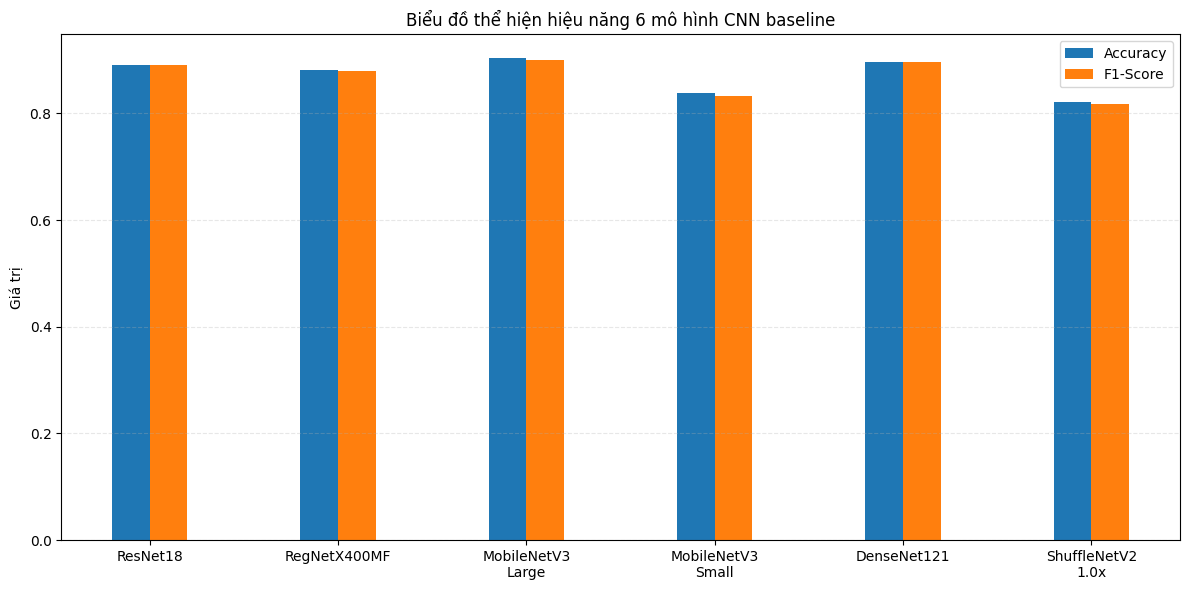
\includegraphics[width=\linewidth]{images/part-02/chap-03/sec-02/CNNBaseline.png}
    \caption{Biểu đồ thể hiện hiệu năng của 6 mô hình CNN baseline}
    \label{fig:CNNBaseline}
\end{figure}

\indent Dựa trên bảng tổng hợp và các biểu đồ thể hiện kết quả trung bình của sáu mô hình CNN baseline, có thể rút ra một số kết luận chính như sau:\vspace{-0.1cm}
\begin{itemize}[label={--}, itemsep=1pt]
    \item MobileNetV3 Large đạt được kết quả trung bình tốt nhất trong bài toán này với Accuracy đạt 0.9028 và F1-Score đạt 0.9006. Mặc dù trước đó DenseNet121 cho ra kết quả tốt nhất, điều này cho thấy sự thích ứng của mô hình MobileNet V3 Large với các tập dữ liệu khác nhau (được drop ngẫu nhiên theo random seed), làm cho kết quả của mô hình vẫn ổn định qua các lần chạy.

    \item DenseNet121, ResNet18 và RegNetX400MF đạt độ chính xác ở mức cao và khá sát nhau, lần lượt là 0.8963, 0.8907 và 0.8806. DenseNet121 vẫn thể hiện ưu thế về khả năng học đặc trưng ở từng lần chạy riêng lẻ, tuy nhiên khi xét trên kết quả trung bình, mô hình này thấp hơn MobileNetV3 Large một khoảng nhỏ. Điều này cho thấy các kiến trúc có quy mô lớn vẫn hoạt động hiệu quả, nhưng chưa hẳn là lựa chọn tối ưu nếu xét đến sự cân bằng giữa hiệu suất và chi phí tính toán.

    \item MobileNetV3 Small và ShuffleNetV2 1.0x đạt kết quả thấp hơn rất nhiều, với độ chính xác lần lượt là 0.8379 và 0.8204. Khoảng cách gần 8\% so với nhóm mô hình dẫn đầu cho thấy việc giản lược mô hình quá mức đã làm hạn chế khả năng nắm bắt các chi tiết, góc cạnh phức tạp, đặc biệt đối với các lớp dữ liệu có bối cảnh hình ảnh tương đồng.
\end{itemize}

Kết quả kiểm thử cho thấy các mô hình CNN baseline, khi chỉ sử dụng thông tin hình ảnh, có thể đạt độ chính xác xấp xỉ \textbf{0.91}. Tuy nhiên, việc khó vượt qua ngưỡng này, cùng với những hạn chế trong việc phân biệt các lớp có mức độ nhập nhằng cao (chẳng hạn như lớp \textit{le-hoi-nghinh-ong}), cho thấy sự cần thiết của việc bổ sung thêm thông tin từ hai phương thức văn bản và âm thanh.
\subsubsection{2.3. Kết quả kiểm thử trên mô hình CNN + MGAT + FastKAN/MLP với toàn bộ phương thức}
\indent\indent Dưới đây là kết quả kiểm thử chi tiết của 12 mô hình CNN backbone + MGAT + FastKAN/MLP với toàn bộ phương thức, trong đó các giá trị được lấy từ lần chạy đạt kết quả cao nhất.\vspace{0.3cm}

%===================================================================
\textbf{* ResNet18 + MGAT + FastKAN/MLP:} 
\begin{table}[H] 
\centering 
\renewcommand{\arraystretch}{1.08} 
\caption{\centering Classification report của FastKAN(1) và MLP(2) trên toàn bộ phương thức với backbone ResNet18} 
\begin{tabular}{lccccccc} 
\hline \textbf{Lớp} & \textbf{P(1)} & \textbf{R(1)} & \textbf{F1(1)} & \textbf{P(2)} & \textbf{R(2)} & \textbf{F1(2)} & \textbf{Support} \\ \hline

cho-noi-cai-rang 
& 1.0000 & 0.9556 & \textbf{0.9773} 
& 0.9333 & 0.9333 & 0.9333 & 45 \\

dua-bo-bay-nui 
& 1.0000 & 1.0000 & \textbf{1.0000} 
& 0.9574 & 1.0000 & 0.9783 & 45 \\

hoi-lim 
& 0.9762 & 0.9111 & \textbf{0.9425} 
& 0.9130 & 0.9333 & 0.9231 & 45 \\

le-hoi-nghinh-ong 
& 0.9000 & 0.8000 & \textbf{0.8471} 
& 0.8261 & 0.8444 & 0.8352 & 45 \\

nghe-dan-tre 
& 1.0000 & 1.0000 & \textbf{1.0000} 
& 0.9565 & 0.9778 & 0.9670 & 45 \\

nghe-det-chieu 
& 0.9574 & 1.0000 & \textbf{0.9783} 
& 0.9348 & 0.9556 & 0.9451 & 45 \\

ok-om-bok 
& 0.9574 & 1.0000 & \textbf{0.9783} 
& 1.0000 & 0.8444 & 0.9157 & 45 \\

via-ba-chua-xu-nui-sam 
& 0.8235 & 0.9333 & \textbf{0.8750} 
& 0.8478 & 0.8667 & 0.8571 & 45 \\ 
\hline

\textbf{Accuracy} 
& & & \textbf{0.9500} 
& & & 0.9194 & 360 \\

\textbf{Macro avg} 
& \textbf{0.9518} & \textbf{0.9500} & \textbf{0.9498} 
& 0.9211 & 0.9194 & 0.9193 & 360 \\

\textbf{Weighted avg} 
& \textbf{0.9518} & \textbf{0.9500} & \textbf{0.9498} 
& 0.9211 & 0.9194 & 0.9193 & 360 \\ 
\hline 
\end{tabular} 
\end{table}

%===================================================================
\textbf{* RegNetX400MF + MGAT + FastKAN/MLP:}
\begin{table}[H]
\centering
\renewcommand{\arraystretch}{1.08}
\caption{\centering Classification report của FastKAN(1) và MLP(2) trên toàn bộ phương thức với backbone RegNetX400MF}
\begin{tabular}{lccccccc}
\hline
\textbf{Lớp} &
\textbf{P(1)} & \textbf{R(1)} & \textbf{F1(1)} &
\textbf{P(2)} & \textbf{R(2)} & \textbf{F1(2)} &
\textbf{Support} \\
\hline

cho-noi-cai-rang
& 0.9778 & 0.9778 & \textbf{0.9778}
& 0.9565 & 0.9778 & 0.9670 & 45 \\

dua-bo-bay-nui
& 1.0000 & 1.0000 & \textbf{1.0000}
& 0.9375 & 1.0000 & 0.9677 & 45 \\

hoi-lim
& 0.8889 & 0.8889 & 0.8889
& 0.9318 & 0.9111 & \textbf{0.9213} & 45 \\

le-hoi-nghinh-ong
& 0.7727 & 0.7556 & 0.7640
& 0.8649 & 0.7111 & \textbf{0.7805} & 45 \\

nghe-dan-tre
& 1.0000 & 1.0000 & \textbf{1.0000}
& 0.9783 & 1.0000 & 0.9890 & 45 \\

nghe-det-chieu
& 0.9778 & 0.9778 & \textbf{0.9778}
& 1.0000 & 0.8889 & 0.9412 & 45 \\

ok-om-bok
& 0.9545 & 0.9333 & 0.9438
& 0.9556 & 0.9556 & \textbf{0.9556} & 45 \\

via-ba-chua-xu-nui-sam
& 0.7660 & 0.8000 & 0.7826
& 0.7593 & 0.9111 & \textbf{0.8283} & 45 \\
\hline

\textbf{Accuracy}
& & & 0.9167
& & & \textbf{0.9194} & 360 \\

\textbf{Macro avg}
& 0.9172 & 0.9167 & 0.9169
& \textbf{0.9230} & \textbf{0.9194} & \textbf{0.9188} & 360 \\

\textbf{Weighted avg}
& 0.9172 & 0.9167 & 0.9169
& \textbf{0.9230} & \textbf{0.9194} & \textbf{0.9188} & 360 \\
\hline
\end{tabular}
\end{table}
%===================================================================
\textbf{* MobileNetV3 Large + MGAT + FastKAN/MLP:}
\begin{table}[H]
\centering
\renewcommand{\arraystretch}{1.08}
\caption{\centering Classification report của FastKAN(1) và MLP(2) trên toàn bộ phương thức với backbone MobileNetV3 Large}
\label{tab:CRMobileNetV3LargeMGATFastKANMLP}
\begin{tabular}{lccccccc}
\hline
\textbf{Lớp} &
\textbf{P(1)} & \textbf{R(1)} & \textbf{F1(1)} &
\textbf{P(2)} & \textbf{R(2)} & \textbf{F1(2)} &
\textbf{Support} \\
\hline
cho-noi-cai-rang
& 0.9184 & 1.0000 & 0.9574
& 0.9778 & 0.9778 & \textbf{0.9778} & 45 \\

dua-bo-bay-nui
& 1.0000 & 1.0000 & \textbf{1.0000}
& 0.9783 & 1.0000 & 0.9890 & 45 \\

hoi-lim
& 0.9111 & 0.9111 & \textbf{0.9111}
& 0.8333 & 0.8889 & 0.8602 & 45 \\

le-hoi-nghinh-ong
& 0.8780 & 0.8000 & \textbf{0.8372}
& 0.8684 & 0.7333 & 0.7952 & 45 \\

nghe-dan-tre
& 1.0000 & 0.9778 & \textbf{0.9888}
& 0.9778 & 0.9778 & 0.9778 & 45 \\

nghe-det-chieu
& 0.9762 & 0.9111 & 0.9425
& 0.9767 & 0.9333 & \textbf{0.9545} & 45 \\

ok-om-bok
& 0.9773 & 0.9556 & \textbf{0.9663}
& 0.9130 & 0.9333 & 0.9231 & 45 \\

via-ba-chua-xu-nui-sam
& 0.8000 & 0.8889 & \textbf{0.8421}
& 0.7551 & 0.8222 & 0.7872 & 45 \\
\hline

\textbf{Accuracy}
& & & {\textbf{0.9306}}
& & & {0.9083} & 360 \\

\textbf{Macro avg}
& \textbf{0.9326} & \textbf{0.9306} & \textbf{0.9307}
& 0.9101 & 0.9083 & 0.9081 & 360 \\

\textbf{Weighted avg}
& \textbf{0.9326} & \textbf{0.9306} & \textbf{0.9307}
& 0.9101 & 0.9083 & 0.9081 & 360 \\
\hline
\end{tabular}
\end{table}
%===================================================================
\textbf{* MobileNetV3 Small + MGAT + FastKAN/MLP:}
\begin{table}[H]
\centering
\renewcommand{\arraystretch}{1.08}
\caption{\centering Classification report của FastKAN(1) và MLP(2) trên toàn bộ phương thức với backbone MobileNetV3 Small}
\begin{tabular}{lccccccc}
\hline
\textbf{Lớp} &
\textbf{P(1)} & \textbf{R(1)} & \textbf{F1(1)} &
\textbf{P(2)} & \textbf{R(2)} & \textbf{F1(2)} &
\textbf{Support} \\
\hline

cho-noi-cai-rang
& 0.9778 & 0.9778 & \textbf{0.9778}
& 0.8980 & 0.9778 & 0.9362 & 45 \\

dua-bo-bay-nui
& 1.0000 & 0.9778 & 0.9888
& 1.0000 & 1.0000 & \textbf{1.0000} & 45 \\

hoi-lim
& 0.9302 & 0.8889 & 0.9091
& 0.9111 & 0.9111 & \textbf{0.9111} & 45 \\

le-hoi-nghinh-ong
& 0.7857 & 0.7333 & 0.7586
& 0.8372 & 0.8000 & \textbf{0.8182} & 45 \\

nghe-dan-tre
& 0.9773 & 0.9556 & 0.9663
& 1.0000 & 0.9778 & \textbf{0.9888} & 45 \\

nghe-det-chieu
& 0.9130 & 0.9333 & 0.9231
& 0.9535 & 0.9111 & \textbf{0.9318} & 45 \\

ok-om-bok
& 0.9565 & 0.9778 & \textbf{0.9670}
& 0.9556 & 0.9556 & 0.9556 & 45 \\

via-ba-chua-xu-nui-sam
& 0.7600 & 0.8444 & 0.8000
& 0.8261 & 0.8444 & \textbf{0.8352} & 45 \\
\hline

\textbf{Accuracy}
& & & 0.9111
& & & \textbf{0.9222} & 360 \\

\textbf{Macro avg}
& 0.9126 & 0.9111 & 0.9113
& \textbf{0.9227} & \textbf{0.9222} & \textbf{0.9221} & 360 \\

\textbf{Weighted avg}
& 0.9126 & 0.9111 & 0.9113
& \textbf{0.9227} & \textbf{0.9222} & \textbf{0.9221} & 360 \\
\hline
\end{tabular}
\end{table}
%===================================================================
\textbf{* DenseNet121 + MGAT + FastKAN/MLP:}
\begin{table}[H]
\centering
\renewcommand{\arraystretch}{1.08}
\caption{\centering Classification report của FastKAN(1) và MLP(2) trên toàn bộ phương thức với backbone DenseNet121}
\begin{tabular}{lccccccc}
\hline
\textbf{Lớp} &
\textbf{P(1)} & \textbf{R(1)} & \textbf{F1(1)} &
\textbf{P(2)} & \textbf{R(2)} & \textbf{F1(2)} &
\textbf{Support} \\
\hline

cho-noi-cai-rang
& 1.0000 & 1.0000 & \textbf{1.0000}
& 0.9565 & 0.9778 & 0.9670 & 45 \\

dua-bo-bay-nui
& 1.0000 & 1.0000 & \textbf{1.0000}
& 1.0000 & 1.0000 & \textbf{1.0000} & 45 \\

hoi-lim
& 0.9302 & 0.8889 & 0.9091
& 0.9149 & 0.9556 & \textbf{0.9348} & 45 \\

le-hoi-nghinh-ong
& 0.8750 & 0.9333 & 0.9032
& 0.9111 & 0.9111 & \textbf{0.9111} & 45 \\

nghe-dan-tre
& 1.0000 & 0.9778 & 0.9888
& 0.9783 & 1.0000 & \textbf{0.9890} & 45 \\

nghe-det-chieu
& 0.9783 & 1.0000 & \textbf{0.9890}
& 1.0000 & 0.9556 & 0.9773 & 45 \\

ok-om-bok
& 0.9318 & 0.9111 & 0.9213
& 0.9333 & 0.9333 & \textbf{0.9333} & 45 \\

via-ba-chua-xu-nui-sam
& 0.9333 & 0.9333 & \textbf{0.9333}
& 0.9302 & 0.8889 & 0.9091 & 45 \\
\hline

\textbf{Accuracy}
& & & \textbf{0.9556}
& & & 0.9528 & 360 \\

\textbf{Macro avg}
& \textbf{0.9561} & \textbf{0.9556} & \textbf{0.9556}
& 0.9530 & 0.9528 & 0.9527 & 360 \\

\textbf{Weighted avg}
& \textbf{0.9561} & \textbf{0.9556} & \textbf{0.9556}
& 0.9530 & 0.9528 & 0.9527 & 360 \\
\hline
\end{tabular}
\end{table}

%===================================================================
\textbf{* ShuffleNetV2 1.0x + MGAT + FastKAN/MLP:}
\begin{table}[H]
\centering
\renewcommand{\arraystretch}{1.08}
\caption{\centering Classification report của FastKAN(1) và MLP(2) trên toàn bộ phương thức với backbone ShuffleNetV2 1.0x}
\begin{tabular}{lccccccc}
\hline
\textbf{Lớp} &
\textbf{P(1)} & \textbf{R(1)} & \textbf{F1(1)} &
\textbf{P(2)} & \textbf{R(2)} & \textbf{F1(2)} &
\textbf{Support} \\
\hline

cho-noi-cai-rang
& 1.0000 & 0.9111 & \textbf{0.9535}
& 0.9556 & 0.9556 & 0.9556 & 45 \\

dua-bo-bay-nui
& 0.9778 & 0.9778 & 0.9778
& 1.0000 & 0.9778 & \textbf{0.9888} & 45 \\

hoi-lim
& 0.8478 & 0.8667 & 0.8571
& 0.8958 & 0.9556 & \textbf{0.9247} & 45 \\

le-hoi-nghinh-ong
& 0.8333 & 0.8889 & \textbf{0.8602}
& 0.8750 & 0.7778 & 0.8235 & 45 \\

nghe-dan-tre
& 1.0000 & 0.9333 & 0.9655
& 0.9556 & 0.9556 & \textbf{0.9556} & 45 \\

nghe-det-chieu
& 0.8800 & 0.9778 & 0.9263
& 0.9565 & 0.9778 & \textbf{0.9670} & 45 \\

ok-om-bok
& 0.8667 & 0.8667 & 0.8667
& 1.0000 & 0.9333 & \textbf{0.9655} & 45 \\

via-ba-chua-xu-nui-sam
& 0.8837 & 0.8444 & \textbf{0.8636}
& 0.8200 & 0.9111 & 0.8632 & 45 \\
\hline

\textbf{Accuracy}
& & & 0.9083
& & & \textbf{0.9306} & 360 \\

\textbf{Macro avg}
& 0.9112 & 0.9083 & 0.9088
& \textbf{0.9323} & \textbf{0.9306} & \textbf{0.9305} & 360 \\

\textbf{Weighted avg}
& 0.9112 & 0.9083 & 0.9088
& \textbf{0.9323} & \textbf{0.9306} & \textbf{0.9305} & 360 \\
\hline
\end{tabular}
\end{table}

\indent Dựa trên kết quả kiểm thử chi tiết của các mô hình CNN backbone kết hợp với MGAT và FastKAN/MLP trên tập dữ liệu kiểm thử với đầy đủ ba phương thức, có thể rút ra một số nhận xét chính như sau:\vspace{-0.1cm}
\begin{itemize}[label={--}, itemsep=1pt]
    \item Hiệu quả của tiếp cận đa phương thức: So với các mô hình CNN baseline chỉ sử dụng thông tin hình ảnh (với Accuracy trung bình xấp xỉ 0.9-0.91), việc tích hợp thêm dữ liệu văn bản và âm thanh thông qua kiến trúc MGAT giúp cải thiện kết quả một cách đáng kể trên hầu hết các backbone. Mức cải thiện này thể hiện rõ nhất ở các lớp có mức độ nhập nhằng cao trong dữ liệu hình ảnh (\textit{le-hoi-nghinh-ong} và \textit{via-ba-chua-xu-nui-sam}), cho thấy vai trò bổ trợ quan trọng của thông tin ngữ nghĩa và âm thanh trong quá trình phân loại.
    
    \item So sánh FastKAN và MLP trên từng backbone:\vspace{-0.1cm}
    \begin{itemize}[label={+}, itemsep=1pt]
        \item ResNet18: FastKAN thể hiện ưu thế rõ rệt so với MLP. Mô hình ResNet18 kết hợp FastKAN đạt độ chính xác 0.95, cao hơn đáng kể so với 0.9194 của MLP. Đặc biệt, tại lớp khó \textit{via-ba-chua-xu-nui-sam}, FastKAN giúp cải thiện Recall từ 0.87 lên 0.93, cho thấy khả năng mô hình hóa các biên quyết định phi tuyến phức tạp hiệu quả hơn so với cấu trúc MLP truyền thống.
        \item DenseNet121: Đây là backbone cho kết quả cao nhất trong toàn bộ các kết quả kiểm thử, với độ chính xác vượt ngưỡng 0.95 ở cả hai bộ phân lớp FastKAN và MLP. So với mô hình CNN baseline đơn phương thức, mức cải thiện đạt được vào khoảng 5\%, cho thấy sự kết hợp giữa biểu diễn đặc trưng mạnh và tích hợp đa phương thức mang lại hiệu quả đáng kể.
        \item MobileNetV3 Large: FastKAN tiếp tục cho thấy lợi thế với Accuracy đạt 0.9306, so với 0.9083 của MLP. Mô hình đạt kết quả gần như tuyệt đối ở lớp \textit{dua-bo-bay-nui}, đồng thời cải thiện đáng kể F1-Score của lớp \textit{le-hoi-nghinh-ong} (0.8372 so với 0.7952). Điều này cho thấy sự kết hợp giữa một backbone gọn nhẹ và một bộ phân lớp có năng lực biểu diễn cao là một hướng tiếp cận tiềm năng.
        \item Các backbone MobileNetV3 Small, ShuffleNetV2 và RegNet: Trong nhóm các kiến trúc gọn nhẹ hơn, MLP cho kết quả tương đương hoặc nhỉnh hơn FastKAN. Chẳng hạn, với ShuffleNetV2 1.0x, MLP đạt độ chính xác 0.9306 trong khi FastKAN đạt 0.9083. Khi đặc trưng đầu vào từ backbone bị nén mạnh và chứa ít thông tin hơn, độ phức tạp cao của FastKAN có thể dẫn đến hiện tượng overfitting nhẹ, trong khi cấu trúc đơn giản của MLP giúp mô hình duy trì khả năng tổng quát hóa tốt hơn.
    \end{itemize}
\end{itemize}

%===================================================================
Dưới đây là bảng tổng hợp và biểu đồ thể hiện kết quả trung bình của tất cả 12 mô hình CNN backbone + MGAT + FastKAN/MLP:
\begin{table}[H]
\centering
\renewcommand{\arraystretch}{1.2}
\setlength{\tabcolsep}{6pt}
\caption{\centering Kết quả kiểm thử trung bình của tất cả các mô hình CNN backbone + MGAT + FastKAN/MLP trên toàn bộ phương thức}
\begin{tabular}{llcccc}
\hline
\textbf{Backbone Model (+ MGAT)} & \textbf{Classifier} & \textbf{Accuracy} & \textbf{Precision} & \textbf{Recall} & \textbf{F1-Score} \\ 
\hline

% ResNet18
\multirow{2}{*}{ResNet18} 
& FastKAN & \textbf{0.9343} & \textbf{0.9358} & \textbf{0.9343} & \textbf{0.9341} \\
& MLP & 0.9000 & 0.9030 & 0.9000 & 0.8996 \\ 
\hline

% RegNetX400MF
\multirow{2}{*}{RegNetX400MF} 
& FastKAN & 0.9074 & 0.9094 & 0.9074 & 0.9071 \\
& MLP & \textbf{0.9092} & \textbf{0.9134} & \textbf{0.9092} & \textbf{0.9090} \\ 
\hline

% MobileNetV3 Large
\multirow{2}{*}{MobileNetV3 Large} 
& FastKAN & \textbf{0.9260} & \textbf{0.9283} & \textbf{0.9260} & \textbf{0.9258} \\
& MLP & 0.9056 & 0.9059 & 0.9056 & 0.9043 \\ 
\hline

% MobileNetV3 Small
\multirow{2}{*}{MobileNetV3 Small} 
& FastKAN & 0.9055 & 0.9111 & 0.9055 & 0.9041 \\
& MLP & \textbf{0.9120} & \textbf{0.9174} & \textbf{0.9120} & \textbf{0.9118} \\ 
\hline

% DenseNet121
\multirow{2}{*}{DenseNet121} 
& FastKAN & \textbf{0.9435} & \textbf{0.9477} & \textbf{0.9435} & \textbf{0.9438} \\
& MLP & 0.9417 & 0.9455 & 0.9417 & 0.9413 \\ 
\hline

% ShuffleNetV2
\multirow{2}{*}{ShuffleNetV2 1.0x} 
& FastKAN & 0.8981 & 0.9007 & 0.8981 & 0.8980 \\
& MLP & \textbf{0.9204} & \textbf{0.9236} & \textbf{0.9204} & \textbf{0.9203} \\ 
\hline

\end{tabular}
\label{tab:avg_performance_comparison}
\end{table}

\begin{figure}[H]
    \centering
    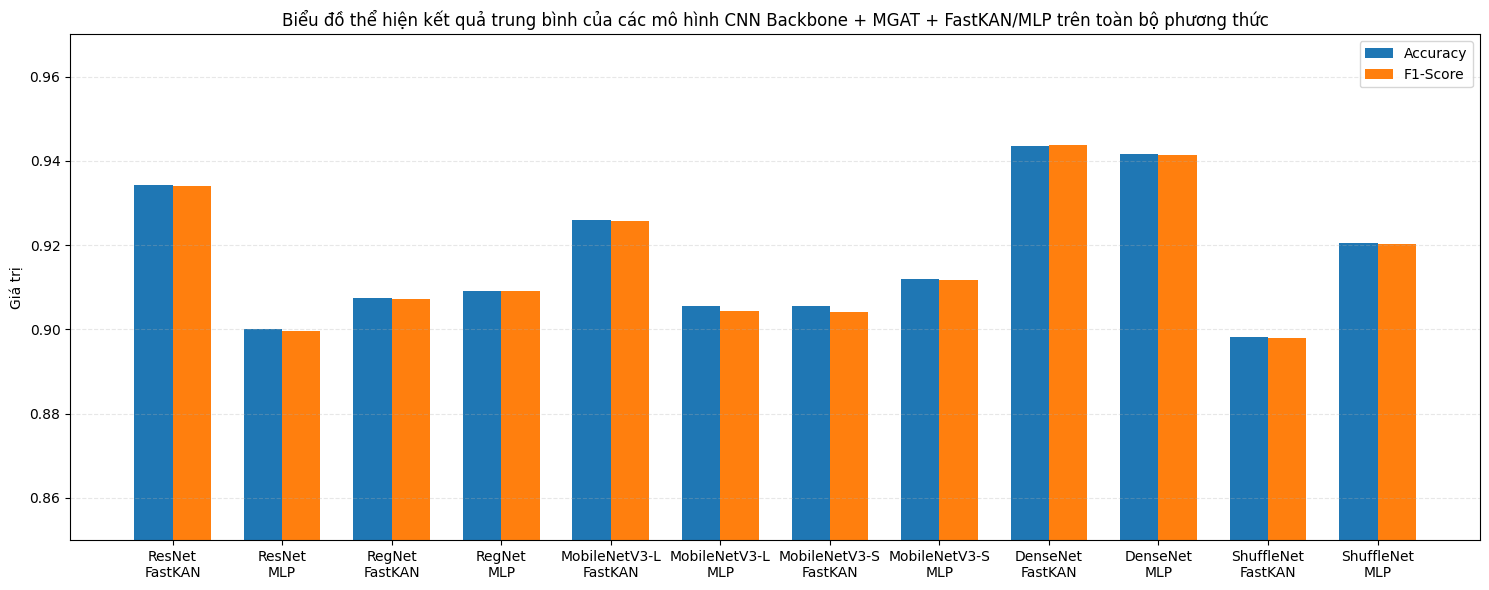
\includegraphics[width=\linewidth]{images/part-02/chap-03/sec-02/PipelineFull.png}
    \caption{\centering Biểu đồ thể hiện kết quả kiểm thử trung bình của tất cả các mô hình CNN backbone + MGAT + FastKAN/MLP trên toàn bộ phương thức}
    \label{fig:KQPipelineFull}
\end{figure}

% \indent Dựa trên bảng tổng hợp và biểu đồ thể hiện kết quả trung bình của 12 mô hình trên toàn bộ phương thức, tôi đưa ra các kết luận sau:\vspace{-0.1cm}
% \begin{itemize}[label={--}, itemsep=1pt]
%     \item \textbf{Khẳng định tính hiệu quả của phương pháp đề xuất:} Hầu hết các mô hình MGAT (dù kết hợp với FastKAN hay MLP) đều vượt qua ngưỡng hiệu năng của CNN Baseline (cao nhất ~0.90). Nổi bật nhất là sự kết hợp DenseNet121 + MGAT + FastKAN đạt tới \textbf{0.9435} và ResNet18 + MGAT + FastKAN đạt \textbf{0.9343}. Điều này chứng minh rằng việc mô hình hóa dữ liệu dưới dạng đồ thị đa phương thức đã thành công trong việc tận dụng thông tin bổ trợ từ văn bản và âm thanh để bù đắp các khoảng trống tri thức mà mô hình đơn phương thức bỏ sót.
%     \item \textbf{Sự tương quan giữa FastKAN và MLP:} Kết quả kiểm thử chỉ ra không có một bộ phân lớp nào là tối ưu cho mọi trường hợp:
%     \begin{itemize}[label={+}, itemsep=1pt]
%         \item \textbf{FastKAN} là lựa chọn tối ưu cho các mô hình có khả năng trích xuất đặc trưng mạnh (backbone lớn/sâu như ResNet, DenseNet, MobileNet Large). Khả năng biểu diễn hàm linh hoạt của KAN giúp khai thác triệt để lượng thông tin phong phú từ các backbone, điều này đã giúp đẩy độ chính xác phân lớp lên mức cao hơn.
%         \item \textbf{MLP} lại là giải pháp an toàn và hiệu quả cho các mô hình gọn nhẹ (backbone nhỏ như MobileNet Small, ShuffleNet). Trong trường hợp tài nguyên tính toán cực kỳ hạn chế, sự kết hợp ShuffleNetV2 + MLP (0.9204) mang lại kết quả rất ấn tượng.
%     \end{itemize}
% \end{itemize}

\indent Dựa trên bảng tổng hợp và các biểu đồ thể hiện kết quả trung bình của 12 mô hình trên toàn bộ phương thức, có thể rút ra những kết luận chính sau:\vspace{-0.1cm}
\begin{itemize}[label={--}, itemsep=1pt]
    \item Khẳng định hiệu quả của phương pháp đề xuất: Phần lớn các mô hình sử dụng MGAT (kết hợp với FastKAN hoặc MLP) cho ra kết quả cao hơn so với mô hình CNN baseline (cao nhất khoảng 0.91). Nổi bật nhất trong số đó là sự kết hợp của mô hình DenseNet121 + MGAT + FastKAN với độ chính xác đạt \textbf{0.9435} và ResNet18 + MGAT + FastKAN đạt 0.9343. Kết quả này cho thấy việc mô hình hóa dữ liệu dưới dạng đồ thị đa phương thức là một phương pháp xử lý hiệu quả các thông tin bổ trợ từ văn bản và âm thanh, qua đó bù đắp những hạn chế của các mô hình đơn phương thức.
    \item Mối quan hệ giữa FastKAN và MLP: Kết quả kiểm thử cho thấy không tồn tại một bộ phân lớp duy nhất có thể tối ưu cho mọi kiến trúc backbone:
    \begin{itemize}[label={+}, itemsep=1pt]
        \item FastKAN phù hợp hơn với các backbone có năng lực trích xuất đặc trưng mạnh (các kiến trúc lớn hoặc sâu như ResNet, DenseNet và MobileNetV3 Large). Nhờ khả năng biểu diễn hàm linh hoạt, FastKAN có thể khai thác hiệu quả lượng thông tin giàu ngữ nghĩa từ các đặc trưng đầu vào, qua đó giúp cải thiện đáng kể độ chính xác phân lớp.
        \item MLP cho ra kết quả ổn định hơn đối với các backbone gọn nhẹ (như MobileNetV3 Small và ShuffleNet). Trong bối cảnh tài nguyên tính toán bị giới hạn nghiêm ngặt, sự kết hợp ShuffleNetV2 + MLP (Accuracy đạt 0.9204) vẫn mang lại kết quả rất ấn tượng..
    \end{itemize}
\end{itemize}
\subsubsection{2.4. Kết quả kiểm thử trên mô hình CNN + MGAT + FastKAN/MLP với hai phương thức (hình ảnh và văn bản)}
\indent\indent Dưới đây là kết quả kiểm thử chi tiết của 12 mô hình CNN backbone + MGAT + FastKAN/MLP với hai phương thức (hình ảnh và văn bản), trong đó các giá trị được lấy từ lần chạy đạt kết quả cao nhất.\vspace{0.3cm}

%===================================================================
\textbf{* ResNet18 + MGAT + FastKAN/MLP:} 
\begin{table}[H]
\centering
\renewcommand{\arraystretch}{1.08}
\caption{\centering Classification report của FastKAN(1) và MLP(2) trên hai phương thức với backbone ResNet18}
\begin{tabular}{lccccccc}
\hline \textbf{Lớp} & \textbf{P(1)} & \textbf{R(1)} & \textbf{F1(1)} & \textbf{P(2)} & \textbf{R(2)} & \textbf{F1(2)} & \textbf{Support} \\ \hline

cho-noi-cai-rang
& 0.9130 & 0.9333 & \textbf{0.9231}
& 1.0000 & 0.7556 & 0.8608 & 45 \\

dua-bo-bay-nui
& 0.9783 & 1.0000 & \textbf{0.9890}
& 0.9574 & 1.0000 & 0.9783 & 45 \\

hoi-lim
& 0.9565 & 0.9778 & \textbf{0.9670}
& 0.9773 & 0.9556 & 0.9663 & 45 \\

le-hoi-nghinh-ong
& 0.8286 & 0.6444 & 0.7250
& 0.8333 & 0.7778 & \textbf{0.8046} & 45 \\

nghe-dan-tre
& 0.9783 & 1.0000 & \textbf{0.9890}
& 0.8654 & 1.0000 & 0.9278 & 45 \\

nghe-det-chieu
& 0.9778 & 0.9778 & \textbf{0.9778}
& 0.9512 & 0.8667 & 0.9070 & 45 \\

ok-om-bok
& 1.0000 & 0.9111 & \textbf{0.9535}
& 0.8400 & 0.9333 & 0.8842 & 45 \\

via-ba-chua-xu-nui-sam
& 0.7091 & 0.8667 & \textbf{0.7800}
& 0.8000 & 0.8889 & 0.8421 & 45 \\
\hline

\textbf{Accuracy}
& & & \textbf{0.9139}
& & & 0.8972 & 360 \\

\textbf{Macro avg}
& \textbf{0.9177} & \textbf{0.9139} & \textbf{0.9130}
& 0.9031 & 0.8972 & 0.8964 & 360 \\

\textbf{Weighted avg}
& \textbf{0.9177} & \textbf{0.9139} & \textbf{0.9130}
& 0.9031 & 0.8972 & 0.8964 & 360 \\
\hline
\end{tabular}
\end{table}

%===================================================================
\newpage
\textbf{* RegNetX400MF + MGAT + FastKAN/MLP:}
\begin{table}[H]
\centering
\renewcommand{\arraystretch}{1.08}
\caption{\centering Classification report của FastKAN(1) và MLP(2) trên hai phương thức với backbone RegNetX400MF}
\begin{tabular}{lccccccc}
\hline \textbf{Lớp} & \textbf{P(1)} & \textbf{R(1)} & \textbf{F1(1)} & \textbf{P(2)} & \textbf{R(2)} & \textbf{F1(2)} & \textbf{Support} \\ \hline

cho-noi-cai-rang
& 0.8600 & 0.9556 & 0.9053 
& 0.9149 & 0.9556 & \textbf{0.9348} & 45 \\

dua-bo-bay-nui 
& 0.9574 & 1.0000 & 0.9783 
& 0.9783 & 1.0000 & \textbf{0.9890} & 45 \\

hoi-lim 
& 0.8113 & 0.9556 & 0.8776 
& 0.9333 & 0.9333 & \textbf{0.9333} & 45 \\

le-hoi-nghinh-ong
& 0.7234 & 0.7556 & 0.7391 
& 0.7500 & 0.8000 & \textbf{0.7742} & 45 \\

nghe-dan-tre
& 1.0000 & 0.9778 & 0.9888 
& 0.9783 & 1.0000 & \textbf{0.9890} & 45 \\

nghe-det-chieu 
& 0.9487 & 0.8222 & 0.8810 
& 0.9556 & 0.9556 & \textbf{0.9556} & 45 \\

ok-om-bok 
& 0.9737 & 0.8222 & 0.8916 
& 0.9545 & 0.9333 & \textbf{0.9438} & 45 \\

via-ba-chua-xu-nui-sam 
& 0.7381 & 0.6889 & 0.7126 
& 0.8718 & 0.7556 & \textbf{0.8095} & 45 \\
\hline

\textbf{Accuracy}
& & & 0.8722
& & & \textbf{0.9167}  & 360 \\

\textbf{Macro avg} 
& 0.8766 & 0.8722 & 0.8718 
& \textbf{0.9171} & \textbf{0.9167} & \textbf{0.9162} & 360 \\

\textbf{Weighted avg}
& 0.8766 & 0.8722 & 0.8718 
& \textbf{0.9171} & \textbf{0.9167} & \textbf{0.9162} & 360 \\
\hline
\end{tabular}
\end{table}
%===================================================================
\textbf{* MobileNetV3 Large + MGAT + FastKAN/MLP:}
\begin{table}[H]
\centering
\renewcommand{\arraystretch}{1.08}
\caption{\centering Classification report của FastKAN(1) và MLP(2) trên hai phương thức với backbone MobileNetV3 Large}
\begin{tabular}{lccccccc}
\hline \textbf{Lớp} & \textbf{P(1)} & \textbf{R(1)} & \textbf{F1(1)} & \textbf{P(2)} & \textbf{R(2)} & \textbf{F1(2)} & \textbf{Support} \\ \hline

cho-noi-cai-rang 
& 0.8824 & 1.0000 & \textbf{0.9375} 
& 0.9149 & 0.9556 & 0.9348 & 45 \\

dua-bo-bay-nui
& 1.0000 & 1.0000 & \textbf{1.0000}
& 1.0000 & 1.0000 & \textbf{1.0000} & 45 \\

hoi-lim 
& 0.9333 & 0.9333 & \textbf{0.9333} 
& 0.8182 & 1.0000 & 0.9000 & 45 \\

le-hoi-nghinh-ong
& 0.9032 & 0.6222 & 0.7368 
& 0.9118 & 0.6889 & \textbf{0.7848} & 45 \\

nghe-dan-tre 
& 0.9783 & 1.0000 & \textbf{0.9890} 
& 0.9783 & 1.0000 & \textbf{0.9890} & 45 \\

nghe-det-chieu 
& 1.0000 & 0.9556 & \textbf{0.9773} 
& 0.9762 & 0.9111 & 0.9425 & 45 \\

ok-om-bok 
& 0.9778 & 0.9778 & \textbf{0.9778} 
& 0.9778 & 0.9778 & \textbf{0.9778} & 45 \\

via-ba-chua-xu-nui-sam
& 0.7222 & 0.8667 & 0.7879 
& 0.8043 & 0.8222 & \textbf{0.8132} & 45 \\
\hline

\textbf{Accuracy}
& & & \textbf{0.9194}
& & & \textbf{0.9194} & 360 \\

\textbf{Macro avg} 
& \textbf{0.9246} & \textbf{0.9194} & 0.9175 
& 0.9227 & \textbf{0.9194} & \textbf{0.9178} & 360 \\

\textbf{Weighted avg} 
& \textbf{0.9246} & \textbf{0.9194} & 0.9175 
& 0.9227 & \textbf{0.9194} & \textbf{0.9178} & 360 \\
\hline
\end{tabular}
\end{table}
%===================================================================
\textbf{* MobileNetV3 Small + MGAT + FastKAN/MLP:}
\begin{table}[H]
\centering
\renewcommand{\arraystretch}{1.08}
\caption{\centering Classification report của FastKAN(1) và MLP(2) trên hai phương thức với backbone MobileNetV3 Small}
\begin{tabular}{lccccccc}
\hline \textbf{Lớp} & \textbf{P(1)} & \textbf{R(1)} & \textbf{F1(1)} & \textbf{P(2)} & \textbf{R(2)} & \textbf{F1(2)} & \textbf{Support} \\ \hline

cho-noi-cai-rang 
& 0.7627 & 1.0000 & 0.8654 
& 0.8980 & 0.9778 & \textbf{0.9362} & 45 \\

dua-bo-bay-nui
& 1.0000 & 0.9556 & \textbf{0.9773} 
& 1.0000 & 0.9556 & \textbf{0.9773} & 45 \\

hoi-lim
& 0.9070 & 0.8667 & 0.8864 
& 0.8936 & 0.9333 & \textbf{0.9130} & 45 \\

le-hoi-nghinh-ong
& 0.7879 & 0.5778 & \textbf{0.6667} 
& 0.7027 & 0.5778 & 0.6341 & 45 \\

nghe-dan-tre
& 0.9574 & 1.0000 & \textbf{0.9783} 
& 1.0000 & 0.9333 & 0.9655 & 45 \\

nghe-det-chieu
& 0.9730 & 0.8000 & 0.8780 
& 0.9333 & 0.9333 & \textbf{0.9333} & 45 \\

ok-om-bok
& 0.9574 & 1.0000 & \textbf{0.9783} 
& 0.9556 & 0.9556 & 0.9556 & 45 \\

via-ba-chua-xu-nui-sam
& 0.6863 & 0.7778 & \textbf{0.7292} 
& 0.6538 & 0.7556 & 0.7010 & 45 \\
\hline

\textbf{Accuracy}
& & & 0.8722
& & & \textbf{0.8778} & 360 \\

\textbf{Macro avg}
& 0.8790 & 0.8722 & 0.8699 
& \textbf{0.8796} & \textbf{0.8778} & \textbf{0.8770} & 360 \\

\textbf{Weighted avg}
& 0.8790 & 0.8722 & 0.8699 
& \textbf{0.8796} & \textbf{0.8778} & \textbf{0.8770} & 360 \\
\hline
\end{tabular}
\end{table}
%===================================================================
\newpage
\textbf{* DenseNet121 + MGAT + FastKAN/MLP:}
\begin{table}[H]
\centering
\renewcommand{\arraystretch}{1.08}
\caption{\centering Classification report của FastKAN(1) và MLP(2) trên hai phương thức với backbone DenseNet121}
\begin{tabular}{lccccccc}
\hline \textbf{Lớp} & \textbf{P(1)} & \textbf{R(1)} & \textbf{F1(1)} & \textbf{P(2)} & \textbf{R(2)} & \textbf{F1(2)} & \textbf{Support} \\ \hline

cho-noi-cai-ran
& 0.9565 & 0.9778 & \textbf{0.9670} 
& 0.9149 & 0.9556 & 0.9348 & 45 \\

dua-bo-bay-nui 
& 0.9375 & 1.0000 & 0.9677 
& 1.0000 & 1.0000 & \textbf{1.0000} & 45 \\

hoi-lim 
& 0.8980 & 0.9778 & \textbf{0.9362} 
& 0.9756 & 0.8889 & 0.9302 & 45 \\

le-hoi-nghinh-ong
& 0.7692 & 0.8889 & 0.8247 
& 0.7843 & 0.8889 & \textbf{0.8333} & 45 \\

nghe-dan-tre
& 0.9783 & 1.0000 & \textbf{0.9890} 
& 1.0000 & 0.9333 & 0.9655 & 45 \\

nghe-det-chieu 
& 1.0000 & 0.9333 & \textbf{0.9655} 
& 0.9111 & 0.9111 & 0.9111 & 45 \\

ok-om-bok
& 0.9744 & 0.8444 & 0.9048 
& 0.9149 & 0.9556 & \textbf{0.9348} & 45 \\

via-ba-chua-xu-nui-sam
& 0.8421 & 0.7111 & 0.7711 
& 0.8571 & 0.8000 & \textbf{0.8276} & 45 \\
\hline

\textbf{Accuracy}
& & & \textbf{0.9167}
& & & \textbf{0.9167} & 360 \\

\textbf{Macro avg} 
& 0.9195 & 0.9167 & 0.9158 
& \textbf{0.9197} & \textbf{0.9167} & \textbf{0.9172} & 360 \\

\textbf{Weighted avg}
& 0.9195 & 0.9167 & 0.9158 
& \textbf{0.9197} & \textbf{0.9167} & \textbf{0.9172} & 360 \\
\hline
\end{tabular}
\end{table}

%===================================================================
\textbf{* ShuffleNetV2 1.0x + MGAT + FastKAN/MLP:}
\begin{table}[H]
\centering
\renewcommand{\arraystretch}{1.08}
\caption{\centering Classification report của FastKAN(1) và MLP(2) trên hai phương thức với backbone ShuffleNetV2 1.0x}
\begin{tabular}{lccccccc}
\hline \textbf{Lớp} & \textbf{P(1)} & \textbf{R(1)} & \textbf{F1(1)} & \textbf{P(2)} & \textbf{R(2)} & \textbf{F1(2)} & \textbf{Support} \\ \hline

cho-noi-cai-rang
& 0.9545 & 0.9333 & \textbf{0.9438}
& 0.9535 & 0.9111 & 0.9318 & 45 \\

dua-bo-bay-nui
& 0.8958 & 0.9556 & 0.9247
& 0.9149 & 0.9556 & \textbf{0.9348} & 45 \\

hoi-lim
& 0.9167 & 0.9778 & \textbf{0.9462}
& 0.8980 & 0.9778 & 0.9362 & 45 \\

le-hoi-nghinh-ong
& 0.8085 & 0.8444 & 0.8261
& 0.8780 & 0.8000 & \textbf{0.8372} & 45 \\

nghe-dan-tre
& 0.9184 & 1.0000 & \textbf{0.9574}
& 0.9767 & 0.9333 & 0.9545 & 45 \\

nghe-det-chieu
& 0.9756 & 0.8889 & \textbf{0.9302}
& 0.8958 & 0.9556 & 0.9247 & 45 \\

ok-om-bok
& 0.9268 & 0.8444 & 0.8837
& 0.9737 & 0.8222 & \textbf{0.8916} & 45 \\

via-ba-chua-xu-nui-sam
& 0.8571 & 0.8000 & \textbf{0.8276}
& 0.7647 & 0.8667 & 0.8125 & 45 \\
\hline

\textbf{Accuracy}
& & & \textbf{0.9056}
& & & 0.9028 & 360 \\

\textbf{Macro avg}
& 0.9067 & \textbf{0.9056} & \textbf{0.9050}
& \textbf{0.9069} & 0.9028 & 0.9029 & 360 \\

\textbf{Weighted avg}
& 0.9067 & \textbf{0.9056} & \textbf{0.9050}
& \textbf{0.9069} & 0.9028 & 0.9029 & 360 \\
\hline
\end{tabular}
\end{table}

\indent Dựa trên kết quả kiểm thử các mô hình chỉ sử dụng hai phương thức, có thể rút ra một số nhận xét chính như sau:\vspace{-0.1cm}
\begin{itemize}[label={--}, itemsep=1pt]
    \item Mức cải thiện rõ rệt ở các mô hình gọn nhẹ: Trái ngược với các kiến trúc quy mô lớn, các backbone nhẹ lại hưởng lợi nhiều hơn từ việc bổ sung thông tin văn bản. Tiêu biểu là ShuffleNetV2 1.0x, từ kết quả thấp nhất ở baseline (0.8222), khi kết hợp với MGAT + FastKAN đã đạt độ chính xác 0.9056; phương án sử dụng MLP cũng cho kết quả tương đương với 0.9028 (mức cải thiện gần 8\%). Tương tự, MobileNetV3 Small cũng cho ra kết quả cao hơn đáng kể khoảng 2.2\% (từ 0.8472 lên 0.8778). Kết quả này cho thấy kiến trúc đồ thị đa phương thức đóng vai trò hiệu quả trong việc bù đắp sự thiếu hụt thông tin biểu diễn của các backbone nhỏ.
    
    \item Hạn chế khi kết hợp RegNetX400MF với FastKAN: Trong khi phần lớn các mô hình đều cải thiện hoặc duy trì kết quả tương đương so với baseline, thì RegNetX400MF kết hợp với FastKAN lại cho thấy sự sụt giảm về độ chính xác (0.8722 so với 0.8806). Ngược lại, khi sử dụng bộ phân lớp MLP, mô hình này đạt kết quả khả quan hơn với độ chính xác 0.9167. Điều này cho thấy đặc trưng trích xuất từ RegNet có thể chưa tương thích tốt với cấu trúc biểu diễn của FastKAN trong không gian đa phương thức.
    
    \item Mức cải thiện hạn chế ở một số mô hình: Đối với các kiến trúc có năng lực trích xuất đặc trưng cao như DenseNet121, ResNet18 và MobileNetV3 Large, kết quả chỉ được cải thiện ở mức khiêm tốn (khoảng 0.3\%–1\% so với baseline). Nguyên nhân có thể là do các mô hình này đã khai thác hiệu quả thông tin hình ảnh ngay từ đầu, khiến dữ liệu văn bản chủ yếu đóng vai trò tinh chỉnh các biên quyết định khó thay vì mang lại sự thay đổi đột phá.
\end{itemize}

%===================================================================
\begin{table}[H]
\centering
\renewcommand{\arraystretch}{1.2}
\setlength{\tabcolsep}{6pt}
\caption{\centering Kết quả kiểm thử trung bình của tất cả các mô hình CNN backbone + MGAT + FastKAN/MLP trên hai phương thức}
\begin{tabular}{llcccc}
\hline
\textbf{Backbone Model (+ MGAT)} & \textbf{Classifier} & \textbf{Accuracy} & \textbf{Precision} & \textbf{Recall} & \textbf{F1-Score} \\
\hline

% ResNet18
\multirow{2}{*}{ResNet18} 
& FastKAN & \textbf{0.8962} & \textbf{0.8993} & \textbf{0.8963} & \textbf{0.8958} \\
& MLP & 0.8843 & 0.8889 & 0.8843 & 0.8834 \\
\hline

% RegNetX400MF
\multirow{2}{*}{RegNetX400MF} 
& FastKAN & 0.8648 & 0.8814 & 0.8648 & 0.8643 \\
& MLP & \textbf{0.8926} & \textbf{0.8942} & \textbf{0.8926}
& \textbf{0.8921} \\
\hline

% MobileNetV3 Large
\multirow{2}{*}{MobileNetV3 Large} 
& FastKAN & 0.9111 & 0.9143 & 0.9111 & 0.9098 \\
& MLP & \textbf{0.9157} & \textbf{0.9177} & \textbf{0.9157} & \textbf{0.9147} \\
\hline

% MobileNetV3 Small
\multirow{2}{*}{MobileNetV3 Small} 
& FastKAN & 0.8583 & 0.8615 & 0.8583 & 0.8557 \\
& MLP & \textbf{0.8694} & \textbf{0.8726} & \textbf{0.8694} & \textbf{0.8687} \\
\hline

% DenseNet121
\multirow{2}{*}{DenseNet121} 
& FastKAN & \textbf{0.9083} & \textbf{0.9102} & \textbf{0.9083} & \textbf{0.9082} \\
& MLP & 0.9037 & 0.9066 & 0.9037 & 0.9028 \\
\hline

% ShuffleNetV2
\multirow{2}{*}{ShuffleNetV2 1.0x} 
& FastKAN & \textbf{0.8982} & 0.8988 & \textbf{0.8982} & \textbf{0.8973} \\
& MLP & 0.8917 & \textbf{0.8989} & 0.8917 & 0.8916 \\
\hline

\end{tabular}
\label{tab:avg_performance_comparison_v2}
\end{table}

\begin{figure}[H]
    \centering
    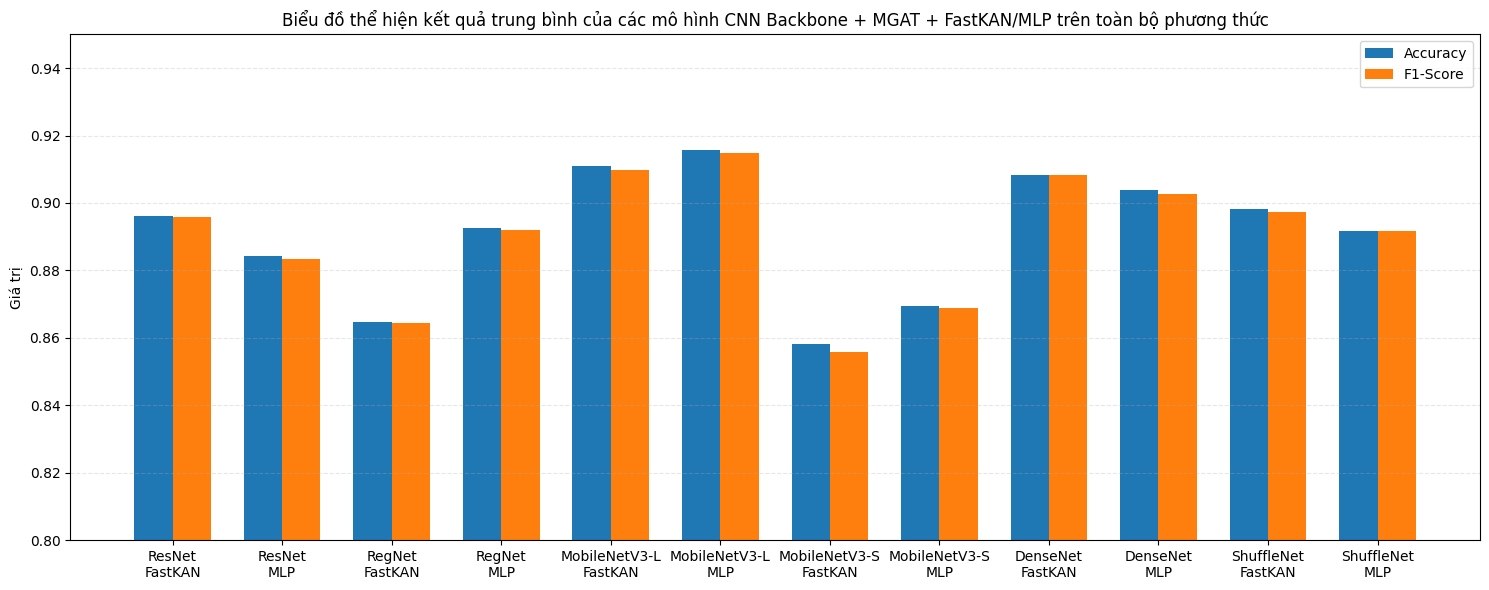
\includegraphics[width=\linewidth]{images/part-02/chap-03/sec-02/PipelineImageText.png}
    \caption{\centering Biểu đồ thể hiện kết quả kiểm thử trung bình của tất cả các mô hình CNN backbone + MGAT + FastKAN/MLP trên hai phương thức}
    \label{fig:KQPipelineImageText}
\end{figure}

\indent Dựa trên bảng tổng hợp và các biểu đồ thể hiện kết quả trung bình của 12 mô hình trên hai phương thức, có thể rút ra các kết luận sau:\vspace{-0.1cm}
\begin{itemize}[label={--}, itemsep=1pt]
    \item Hiệu quả giới hạn của FastKAN trong kịch bản hai phương thức: So với mức cải thiện rõ rệt khi sử dụng đầy đủ ba phương thức (chẳng hạn ResNet18 tăng hơn 3\% so với MLP), thì trong kịch bản chỉ sử dụng hai phương thức, lợi thế của FastKAN thể hiện không rõ ràng, với mức cải thiện chỉ khoảng \textasciitilde 1\%. Điều này cho thấy FastKAN cần một không gian đặc trưng đầu vào đủ phong phú và đa dạng để khai thác hiệu quả khả năng xấp xỉ hàm phi tuyến. Khi thiếu đi thông tin âm thanh, không gian biểu diễn bị thu hẹp, các quan hệ ngữ nghĩa trở nên đơn giản hơn, khiến kiến trúc FastKAN chưa được tận dụng triệt để.

    \item Tính ổn định của MLP trên các backbone MobileNet và RegNet: Với các backbone thuộc dòng MobileNetV3 và RegNetX400MF, MLP cho kết quả ổn định hơn hoặc nhỉnh hơn so với FastKAN. Điển hình là RegNetX400MF, khi kết hợp với MLP đạt độ chính xác 0.8926, cao hơn đáng kể so với 0.8648 của FastKAN. Kết quả này cho thấy đối với dạng đặc trưng được trích xuất từ các backbone này, cấu trúc tuyến tính tương đối đơn giản của MLP phù hợp hơn và ít rủi ro hơn, đồng thời giúp mô hình hội tụ ổn định trong không gian đa phương thức bị rút gọn.
    
    \item Vai trò quan trọng của dữ liệu âm thanh: Mặc dù các mô hình chỉ sử dụng hai phương thức đã cải thiện được kết quả so với CNN Baseline, nhưng khi so sánh với kết quả sử dụng đầy đủ ba phương thức (Mục 2.3), vẫn tồn tại sự chênh lệch đáng kể về độ chính xác (thấp hơn khoảng 2–3\%). Khoảng cách này là minh chứng cho thấy, đối với các bài toán nhận dạng ICH mang tính trình diễn hoặc lễ hội, thông tin từ kênh âm thanh là thành phần quan trọng giúp hoàn thiện biểu diễn ngữ nghĩa và nâng cao hiệu năng tổng thể của hệ thống.
\end{itemize}
\subsubsection{2.5. Kết quả kiểm thử trên mô hình CNN + MGAT + mô hình phân lớp truyền thống với toàn bộ phương thức}
\indent\indent Nhằm đánh giá một cách khách quan chất lượng của các đặc trưng (features) được học bởi kiến trúc đồ thị, đề tài tiến hành thực hiện một thực nghiệm bổ sung, trong đó bộ phân lớp học sâu (FastKAN/MLP) được thay thế bằng các thuật toán máy học truyền thống.\vspace{0.3cm}

Đối với các mô hình máy học truyền thống, quá trình huấn luyện được thực hiện trên các đặc trưng đã được trích xuất sẵn từ mô hình học sâu, bằng cách dùng mô hình CNN backbone + MGAT + FastKAN/MLP đạt kết quả kiểm thử tốt nhất được sử dụng làm bộ mã hóa bằng cách loại bỏ tầng phân lớp cuối cùng. Vector đặc trưng đại diện cho mỗi mẫu đồ thị được xây dựng bằng cách lấy trung bình các vector đặc trưng của toàn bộ các đỉnh thành phần, từ đó thu được một vector đặc trưng có số chiều là 512. Trước khi đưa vào huấn luyện, các vector đặc trưng này được chuẩn hóa bằng kỹ thuật \textit{StandardScaler} nhằm giảm thiểu sự chênh lệch về độ lớn giữa các chiều, giúp các thuật toán máy học truyền thống hoạt động ổn định và hiệu quả hơn. Sáu mô hình máy học truyền thống được lựa chọn để đánh giá bao gồm: KNN, Naive Bayes, Decision Tree, Random Forest, Logistic Regression và Linear SVC.\vspace{0.3cm}

\newpage
Bảng số liệu và các biểu đồ dưới đây trình bày kết quả kiểm thử trung bình của các mô hình máy học truyền thống:
\begin{table}[H]
\centering
\caption{\centering Kết quả kiểm thử trung bình của các mô hình truyền thống (sử dụng đặc trưng từ DenseNet121 + MGAT + FastKAN)}
\label{tab:TraditionalModelsSummary}
\renewcommand{\arraystretch}{1.15}
\begin{tabular}{lcccc}
\hline
\textbf{Mô hình} & \textbf{Accuracy} & \textbf{Precision} & \textbf{Recall} & \textbf{F1-Score} \\
\hline
KNN (k = 1)                   & 0.8213 & 0.8289 & 0.8213 & 0.8022 \\
Gaussian NB                   & 0.7306 & 0.7210 & 0.7306 & 0.7142 \\
Decision Tree (max\_depth = 10) & 0.7556 & 0.7656 & 0.7556 & 0.7412 \\
Random Forest (n\_estimators = 20) & 0.8083 & 0.8108 & 0.8083 & 0.7859 \\
Logistic Regression (C = 10)      & 0.8370 & 0.8419 & 0.8370 & 0.8272 \\
Linear SVC (C = 0.01)             & 0.8676 & 0.8696 & 0.8676 & 0.8649 \\
\hline
{DenseNet121 + MGAT + FastKAN} & \textbf{0.9435} & \textbf{0.9477} & \textbf{0.9435} & \textbf{0.9438} \\
\hline
\end{tabular}
\end{table}

\begin{figure}[H]
    \centering
    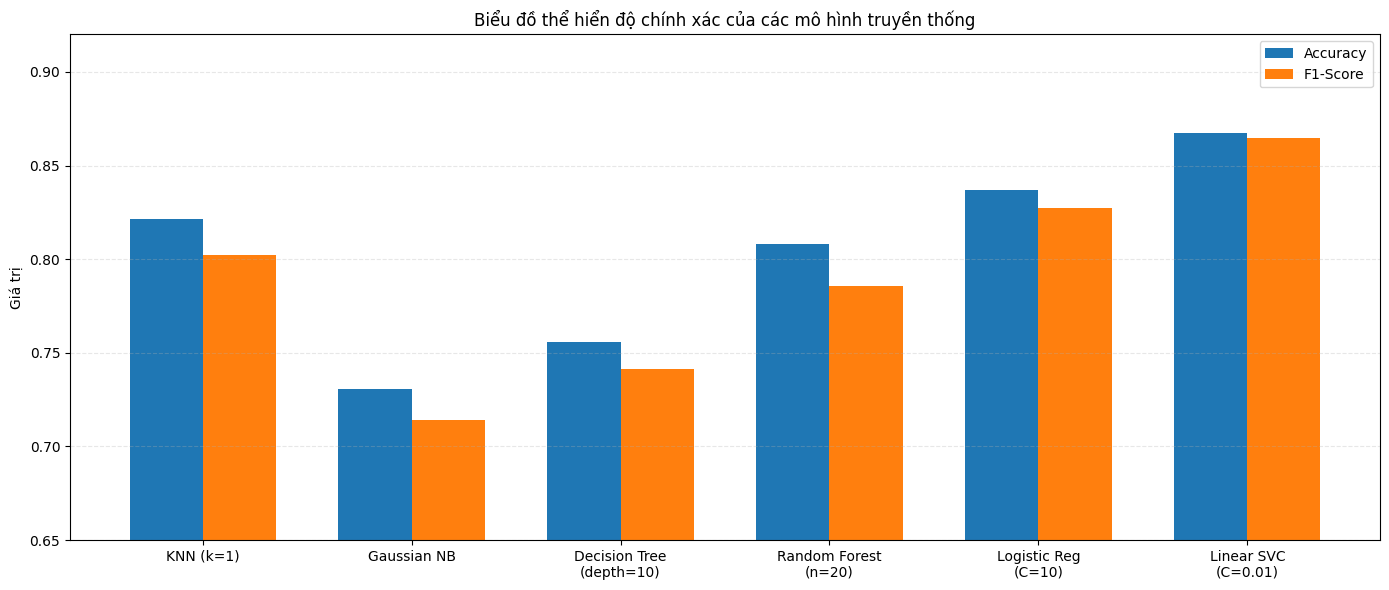
\includegraphics[width=\linewidth]{images/part-02/chap-03/sec-02/Tradition.png}
    \caption{\centering Biểu đồ thể hiện kết quả kiểm thử trung bình của các mô hình truyền thống (sử dụng đặc trưng từ DenseNet121 + MGAT + FastKAN)}
    \label{fig:KQTradition}
\end{figure}

\indent Dựa trên số liệu thu được từ bảng kết quả kiểm thử trung bình của các mô hình máy học truyền thống, có thể rút ra một số nhận xét chính như sau:\vspace{-0.1cm}
\begin{itemize}[label={--}, itemsep=1pt]
    \item Khả năng phân tách tuyến tính của không gian đặc trưng: Kết quả đạt được với Linear SVC (độ chính xác 0.8676) cho thấy các vector đặc trưng đầu ra từ tầng MGAT có mức độ phân tách tuyến tính tương đối tốt. Điều này cho thấy các mẫu dữ liệu cùng lớp có xu hướng được gom cụm trong không gian đặc trưng, tạo điều kiện thuận lợi cho các bộ phân lớp tuyến tính hoạt động hiệu quả.
    
    \item Vai trò trích xuất và tổng hợp đặc trưng của MGAT: Các kết quả kiểm thử đã cho thấy rằng kiến trúc MGAT tổng hợp thông tin từ nhiều phương thức dữ liệu rời rạc (hình ảnh, văn bản và âm thanh) thành các vector biểu diễn ngữ nghĩa thống nhất rất hiệu quả, trước khi được đưa vào các bộ phân lớp ở giai đoạn cuối.
    
    \item So sánh với FastKAN: Mặc dù Linear SVC cho kết quả khả quan, vẫn còn tồn tại một khoảng cách đáng kể về độ chính xác (khoảng 7–8\%) khi so sánh với FastKAN (đạt 0.9435). Sự chênh lệch này thể hiện hạn chế của các mô hình tuyến tính trong việc xử lý các biên quyết định phức tạp. Đối với dữ liệu ICH, nơi tồn tại nhiều mẫu có mức độ nhập nhằng cao, các bộ phân lớp phi tuyến với khả năng biểu diễn linh hoạt như FastKAN sẽ phù hợp hơn so với các mô hình máy học truyền thống.
\end{itemize}

